\begin{figure}[!ht]
\centering
\resizebox{1.0\columnwidth}{!}{
\begin{tabular}{ccc}
 %%%%%%%%%%%%%%%%%%%%%%%%%%%%%% Main Graph %%%%%%%%%%%%%%%%%%%%%%%%%%%%%%
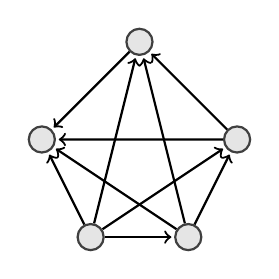
\begin{tikzpicture}[shorten >=1pt,->,scale=0.62]  
        \tikzstyle{sentence}=[circle,thick,draw=black!75,fill=black!10,minimum size=2mm]
        \tikzstyle{edge}=[draw, thick]
       \begin{scope}
         \node [sentence] (s1) at (1,0) {\tiny{}};
         \node [sentence] (s2) at (3,0) {\tiny{}};
         \node [sentence] (s3) at (4,2) {\tiny{}}; 
         \node [sentence] (s4) at (2,4) {\tiny{}}; 
         \node [sentence] (s5) at (0,2) {\tiny{}}; 
         \path[edge] (s1) edge [above] node[font=\tiny] {} (s2);
         \path[edge] (s1) edge [above] node[font=\tiny] {} (s3);
         \path[edge] (s1) edge [above] node[font=\tiny] {} (s4);
         \path[edge] (s1) edge [above] node[font=\tiny] {} (s5);
         
         \path[edge] (s2) edge [above] node[font=\tiny] {} (s3);
         \path[edge] (s2) edge [above] node[font=\tiny] {} (s4);
         \path[edge] (s2) edge [above] node[font=\tiny] {} (s5);
         
         \path[edge] (s3) edge [above] node[font=\tiny] {} (s4);
         \path[edge] (s3) edge [above] node[font=\tiny] {} (s5);
         
         \path[edge] (s4) edge [above] node[font=\tiny] {} (s5);
         
        \end{scope}        
      \end{tikzpicture}
&
%%%%%%%%%%%%%%%%%%%%%%%%%%%%%% Subgraph %%%%%%%%%%%%%%%%%%%%%%%%%%%%%%
 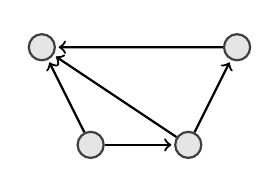
\begin{tikzpicture}[shorten >=1pt,->,scale=0.62]  
        \tikzstyle{sentence}=[circle,thick,draw=black!75,fill=black!10,minimum size=2mm]
        \tikzstyle{edge}=[draw, thick]
       \begin{scope}
         \node [sentence] (s1) at (1,0) {\tiny{}};
         \node [sentence] (s2) at (3,0) {\tiny{}};
         \node [sentence] (s3) at (4,2) {\tiny{}}; 
         \node [sentence] (s5) at (0,2) {\tiny{}}; 

         \path[edge] (s1) edge [above] node[font=\tiny] {} (s2);
         
         \path[edge] (s1) edge [above] node[font=\tiny] {} (s5);
         
         \path[edge] (s2) edge [above] node[font=\tiny] {} (s3);
         \path[edge] (s2) edge [above] node[font=\tiny] {} (s5);
         

         \path[edge] (s3) edge [above] node[font=\tiny] {} (s5);
         
        \end{scope}        
      \end{tikzpicture}

&
 %%%%%%%%%%%%%%%%%%%%%%%%%%%%%% Induced Subgraph %%%%%%%%%%%%%%%%%%%%%%%%%%%%%%
 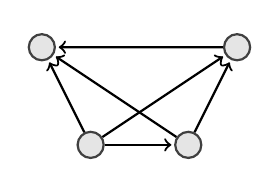
\begin{tikzpicture}[shorten >=1pt,->,scale=0.62]  
        \tikzstyle{sentence}=[circle,thick,draw=black!75,fill=black!10,minimum size=2mm]
        \tikzstyle{edge}=[draw, thick]
       \begin{scope}
         \node [sentence] (s1) at (1,0) {\tiny{}};
         \node [sentence] (s2) at (3,0) {\tiny{}};
         \node [sentence] (s3) at (4,2) {\tiny{}}; 
         \node [sentence] (s5) at (0,2) {\tiny{}}; 

         \path[edge] (s1) edge [above] node[font=\tiny] {} (s2);
         \path[edge] (s1) edge [above] node[font=\tiny] {} (s3);
         \path[edge] (s1) edge [above] node[font=\tiny] {} (s5);
         
         \path[edge] (s2) edge [above] node[font=\tiny] {} (s3);
         \path[edge] (s2) edge [above] node[font=\tiny] {} (s5);
         

         \path[edge] (s3) edge [above] node[font=\tiny] {} (s5);
         
        \end{scope}        
      \end{tikzpicture}
      
\\

\scriptsize{(a)} & \scriptsize{(b)} & \scriptsize{(c)}
                 

\end{tabular}
}
\caption{Both graphs (b) and (c) are subgraphs of (a). Only (c) is
  an induced subgraph of (a).}
\label{f:induced_subgraphs}
\end{figure}